\documentclass{sig-alternate}

\usepackage[utf8]{inputenc}
\usepackage[activate=compatibility]{microtype}

% autoref command
\usepackage[hyphens]{url}
\usepackage[pdftex,urlcolor=black,colorlinks=true,linkcolor=black,citecolor=black]{hyperref}
\def\sectionautorefname{Section}
\def\subsectionautorefname{Subsection}
\def\subfigureautorefname{Subfigure}

\usepackage{setspace}
\usepackage{siunitx}

% Graphics
\usepackage{graphicx}
\usepackage{subfig}
\usepackage[font=small]{caption}
\captionsetup[figure]{name=Figure}
\usepackage{subcaption}

\usepackage{amsmath}
\usepackage{enumitem}
\usepackage{pbox}
\usepackage{color}
\definecolor{light-gray}{gray}{0.8}

% todo macro
\usepackage{color}
\newcommand{\todo}[1]{\noindent\textcolor{red}{{\bf \{TODO}: #1{\bf \}}}}

% listings and Verbatim environment
\usepackage{fancyvrb}
\usepackage{relsize}
\usepackage{listings}
\usepackage{verbatim}
\newcommand{\defaultlistingsize}{\fontsize{8pt}{9.5pt}}
\newcommand{\inlinelistingsize}{\fontsize{8pt}{11pt}}
\newcommand{\smalllistingsize}{\fontsize{7.5pt}{9.5pt}}
\newcommand{\listingsize}{\defaultlistingsize}
\RecustomVerbatimCommand{\Verb}{Verb}{fontsize=\inlinelistingsize}
\RecustomVerbatimEnvironment{Verbatim}{Verbatim}{fontsize=\defaultlistingsize}
\lstset{frame=lines,captionpos=b,numberbychapter=false,escapechar=§,
        aboveskip=2em,belowskip=1em,abovecaptionskip=0.5em,belowcaptionskip=0.5em,
        framexbottommargin=-1em,basicstyle=\ttfamily\listingsize\selectfont}

% use Courier from this point onward
\let\oldttdefault\ttdefault
\renewcommand{\ttdefault}{pcr}
\let\oldurl\url
\renewcommand{\url}[1]{\inlinelistingsize\oldurl{#1}}

\lstdefinelanguage{JavaScript}{
  keywords={push, typeof, new, true, false, catch, function, return, null, catch, switch, var, if, in, while, do, else, case, break},
  keywordstyle=\bfseries,
  ndkeywords={class, export, boolean, throw, implements, import, this},
  ndkeywordstyle=\color{darkgray}\bfseries,
  identifierstyle=\color{black},
  sensitive=false,
  comment=[l]{//},
  morecomment=[s]{/*}{*/},
  commentstyle=\color{darkgray},
  stringstyle=\color{red},
  morestring=[b]',
  morestring=[b]"
}

% linewrap symbol
\definecolor{grey}{RGB}{130,130,130}
\newcommand{\linewrap}{\raisebox{-.6ex}{\textcolor{grey}{$\hookleftarrow$}}}

\hyphenation{}

\begin{document}

\title{Analytics of Realtime Soccer Match Sensor Data with JavaScript and WebGL---Reprocessed and Visualized for Web Browser or Command Line Consumption}

\numberofauthors{1}\author{
\alignauthor
Martin Kleppe\\
  \affaddr{Ubilabs GmbH}\\
  \affaddr{Juliusstr. 25}\\
  \affaddr{22769 Hamburg, Germany}\\
  \email{kleppe@ubilabs.net}
}
\maketitle

\begin{abstract}
In this paper, we report on a~Web application 
with an additional command line interface
capable of providing complex analyses
over high velocity soccer match sensor data
that was implemented in JavaScript
and the Web Graphics Library~(WebGL).
This application visualizes analysis results graphically
in the Web browser and in parallel also
streams aggregated statistics in realtime
to a~command line interface.
The data analyzed in this paper consists of raw sensor data
that was recorded during an actual soccer match
using wireless sensors embedded in the ball
and the players' shoes.
The thereof generated realtime analyses are twofold:
on the one hand, they focus on the continuous computation of statistics
such as ball possession, shots on goal, or player of the match,
which is relevant to passive spectators like fans in a~stadium
or TV viewers at home.
On the other hand, they focus on active observers of the match
like team coaches or team managers that require more detailed analyses
like running path visualizations, position heat maps, \emph{etc.}
\end{abstract}

\keywords{Realtime Analyses, Sensor Data, Data Streams, JavaScript, WebGL, Command Line Interface, Sports, Soccer}

\section{Introduction}

Detailed sports game analyses are of high interest and
relevance in today’s professional sports leagues.
Spectators are provided with additional statistics
such as the number of shots on the goal, movement analyses,
or percentage of ball possession per player or team.
Furthermore, more detailed statistics provide useful information
for coaches and team managers about players' performance
during the match or in certain situations
and also give insights about opponents,
which could lead to modification in tactics.
Although automated solutions
such as high resolution video analyses are desirable
as they generate the required detailed statistics quickly,
at present, most sports game statistics are still processed manually.
Unfortunately, insights gained through image-based solutions
are limited by image resolution, frame rate, and last not least
prohibitive costs.
For The~ACM~DEBS~2013 Grand Challenge,%
\footnote{\url{http://www.orgs.ttu.edu/debs2013/}}
the Fraunhofer Institute for Integrated Circuits~(IIS)%
\footnote{\url{http://www.iis.fraunhofer.de/en/profil.html}}
have set up a realtime locating system on a soccer field
in a~stadium in Nuremberg, Germany.
Every player and the ball were equipped with wireless sensors
that produce high velocity sensor data at a~total rate
of about 15,000 position events per second.

In the following, we will outline our submission to the challenge
that uses continuous computation of statistics in JavaScript
to generate interactive visualizations and realtime analyses
of the game such as ball possession, shots on goal,
running analyses of all players and the two teams.
The chosen approach can be called \emph{hybrid},
as the same system is used to visualize the game in a~Web browser
and to output multiple event streams on the file system.

The remainder of this paper is structured as follows.
We briefly have a~look at related work in \autoref{sec:related-work}.
In \autoref{sec:methodology}, we outline
the methodology of the chosen approach.
\autoref{sec:implementation-details}
is dedicated to the implementation details.
We conclude with an outlook on future work in \autoref{sec:conclusions-future-work}.

\section{Related Work}
\label{sec:related-work}

Automated sport analyses heavily depend on video systems
that capture the game, compute differences between images
and then use the remaining color information
to track players and ball.
Another approach is to equip the players with sensors
that collect position data over time.
That data can be combined with video processing for instance,
to select and zoom in on a situation where a certain player
is within the opponent’s penalty area.
Additionally, biometric sensors that collect information
about the players condition---such as heartbeat
and body temperature---provide data that is used
to analyze the performance during the game.
Spatial game analytics (\emph{e.g.}, heat maps
that display the players’ distribution over time)
are one of the most useful applications,
because they can be used to optimize the team distribution
for a specific game.

Using JavaScript to analyze that amount of data in real-time
was not possible until Node.js,
which is built on top of Google's open source JavaScript engine V8
has proven that it is suitable to build
high-performance network programs
because of its event-driven and non-blocking nature.
Furthermore, HTML5 features, such as Canvas and WebSockets
are used for tools like real-time monitoring systems.
When visualizing three dimensional content,
WebGL---a web standard for a low-level 3D graphics API
based on OpenGL ES 2.0---is ideal to render the objects
in the browser.
It is used for MMOGs (Massively Multiplayer Online Games),
efficient rendering of 3D models
and interactive visualization of volumetric data.

\section{Methodology}
\label{sec:methodology}

The following submission for the ACM DEBS 2013 Grand Challenge
started with the question: ``Is it possible to read and analyze
the provided input data stream and visualize it in the browser''?
The first tests turned out that parsing the file
and simply displaying the positions of all players
and balls in 3D is possible with twenty times the actual speed,
that means, a minute of the real game is replayed
within just three seconds.
This leaves enough time to make additional calculations.
The two teams and the ball can easily be recognized
by using different colors for each.
Additionally the playing field and goals are drawn
to visually check different game situation.

The second step was to implement the required queries.
For every information a visual element was added
to the browser interface to keep track of the computations
and avoid gross errors.
These include: A tracing line for the ball movement,
the list of players with stats about ball possession,
colorized sparklines for running analyses,
the precalculated ball path, the possible hit target,
highlight of current player, an animated acceleration bar
and the current time.

As the application has to deal with large data sets,
it is critical to observe the internally used memory.
The Chrome Developer Tools Timeline Panel was used
to detect if the scripts result into an increasing usage
and then the memory leaks were evaluated and removed.

After all parts were included, the original code
was extended to also run via the command line
without the need of a browser.
Therefore a bridge was created to either render HTML
or output several streams if executed via the command line.
These streams can written to a file or distributed via WebSockets.
The result is a hybrid application that does both:
visualize the match in a browser or share aggregated results
via the network.

\section{Implementation Details}
\label{sec:implementation-details}

Data: The original data-stream was captured during the game
and results in a 4.62 GB CSV input file.
Position updates for sensors in players’ shoes
and goalkeepers’ hands are provided with a frequency of 200Hz.
The sensors in all balls update with 2000Hz.
A record contains the following data:
sensor id, timestamp in picoseconds, position
(in a three-dimensional coordinate system) of the sensor
in mm, |v| (in \SI{}{\micro\metre}/s), vx, vy, vz
describe direction by a vector,
and |a| (in \SI{}{\micro\metre}/s$\square$), ax, ay, az describe the absolute acceleration
and its constituents in three dimensions.

Queries: Based on this data, the following queries are required
for the ACM DEBS 2013 Grand Challenge:
Running analysis, ball possession, heat maps and shots on goal.
Furthermore, goal detection and when the ball is out were included.

Analysis: All entries of the original data stream are distributed
to several JavaScript objects based on a mapping table
that includes more information about the sensor type.
Whenever a ball position update was detected,
the system uses the last known position to check
for a goal or whether the ball has left the field.
If the ball acceleration peaks, it detects the associated player
and computes the shot target
based on the current speed vector and gravity.
Position updates for all players are collected
to result into running statistics and heat map calculations.

Performance: To optimize performance
and to avoid long running scripts,
plain JavaScript with almost zero dependencies was used.
The only exceptions are the library fishbone.js
and Three.js---a wrapper that handles WebGL.
The code was organized into two kinds of modules:
Simple class-like modules with prototype-based inheritance
that were used for fast-changing game objects
like players or ball
and modules that handle events between these objects
and the streams.
A centralized runner script handles
most of the time-consuming calculations within a flat lexical scope
to avoid nested function and variable lookups.
This was especially critical for large loops
that occur when the input stream emits new records.

Aggregations: Whenever an update of one of the balls is detected,
the program evaluates if this ball is active
by comparing the position with the field’s bounds.
Then the nearest player is selected
and if the ball’s acceleration peaks,
shots on goal and ball possessions
(per player and team) are evaluated.
With a frequency of 50Hz, the player’s current position
is recorded into a large array to generate running statistics
and heat maps based on different time frames
(1, 5, 20 minutes and the whole game).
This is done by looping through the records
multiple times per interval
and comparing all dimensions to create aggregated values.

Visualization: To visualize the results in the browser,
position properties of JavaScript objects are updated
as new data arrives---and because WebGL is a state machine,
it handles these updates very fast.
Geometries for sensors are displayed as colored cubes,
the field and ball paths are simple polylines
and the heat map is a particle system.
It uses rectangular sprites, because the rendering performance
of 2D sprites is way better than updating complex geometries.
The list of players is drawn as an unordered HTML list
and colors are assigned via CSS.
The color-coded sparkline graph the end of each list item
is drawn using HTML5 Canvas,
which results in a better performance than plain HTML,
SVG and WebGL, as it generates stateless bitmaps.

Streams: Output for the command-line version was implemented
using file streams: For every calculation that emits events,
a writable stream is created in Node.js.
The current implementation pipes the output to multiple files
on the hard disk, each for every type:
Player running analysis (1 stream),
aggregate running statistics (4 time frames),
player ball possession (1 stream),
team ball possession (1 stream),
heatmaps (4 time frames) and shot on goals (1 stream).
This results into a total of 12 files written to disk.

\begin{figure*}[t!]
  \centering
  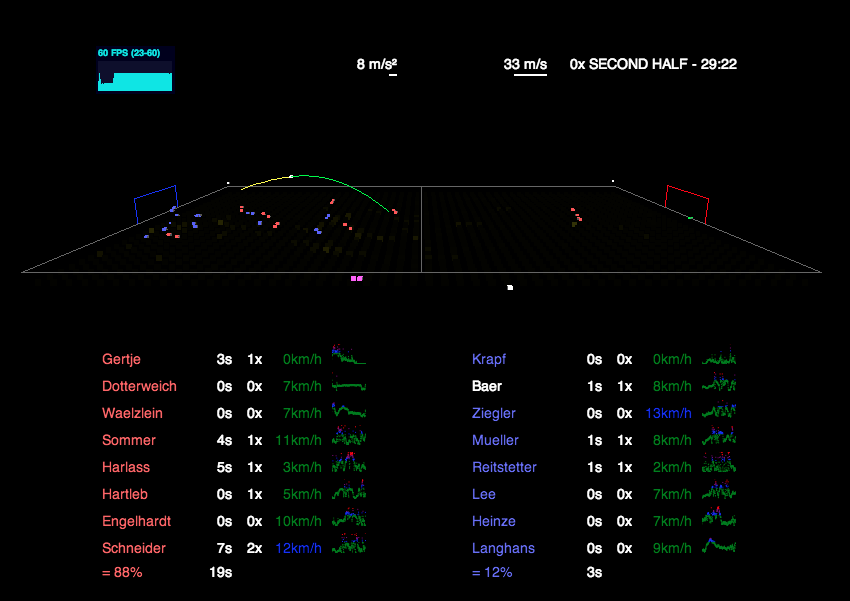
\includegraphics[width=\linewidth]{soccer.png}
  \caption{Screenshot}
  \label{fig:screenshot}
\end{figure*}

\section{Conclusions and Future Work}
\label{sec:conclusions-future-work}

In the first evaluation phase it turned out
that modern JavaScript engines such as V8
are well suited to process large amount of data in real-time.
With the hybrid model it is possible to analyze a full soccer match
on the command line and visualize it in the browser.
HTML5 features such as Canvas and WebGL draw graphics
without any noticeable performance degradation
and the event-driven, non-blocking I/O model of Node.js
is an efficient way to read, process and write data.

As mentioned above, the current implementation
outputs all streams to the file system,
but using the abstract stream pattern in Node.js,
they can be piped to other types of streams such as WebSockets.
A possible use case are mobile devices with limited storage
and computing power.
They connect to the main server via a socket connection
and receive only small chunks of data that are necessary
to render relevant information.
Coaches and team members could benefit from such a solution
for mobile devices, because they are small and portable.

This available type of system can also be ported
to other ball team sports, \emph{e.g.}, American football,
rugby or basketball.
Further work might include more automatic analyses,
such as number of corner shots, passes and duel statistics.
If combined with additional biometric sensor data (pulse, power)
it will give insights to the current player’s condition
or even his progress during a whole season.

\section*{Acknowledgments}
Ubilabs? Thomas Steiner, Klaus Trainer, Michael Pletziger, Jens Wille, Samuel Oey, Robert Katzki

\bibliographystyle{abbrv}
\bibliography{soccer-debs-challenge}

\end{document}